\chapter{Condizionamento dell'Ingresso}

%--------------------------------------------------------------------------------------------

\section{Convertitore Lineare-Esponenziale}

%--------------------------------------------------------------------------------------------

Vogliamo ora analizzare il circuto che soddisfa la specifica sulla modalità $1V/Octave$
dell'ingresso, ovvero il circuito in grado di convertire una tensione lineare in una
esponenziale.

Il circuito utilizzato è molto diffuso in questo tipo di applicazioni, si può infatti
trovare in molti siti di DIY come quello di René Schmitz \cite{expo_converter}, personaggio
molto noto tra gli appassionati di sintetizzatori musicali fai-da-te.

%--------------------------------------------------------------------------------------------

\subsection*{Analisi del Circuito}

%--------------------------------------------------------------------------------------------

Per l'applicazione si sfrutta la caratteristica esponenziale intrinseca del transistor
bipolare:

\begin{displaymath}
    I_e\approx I_c=I_se^{\left(\frac{V_{be}}{V_T}-1\right)}
    \approx I_se^{\left(\frac{V_{be}}{V_T}\right)}\ [A]
\end{displaymath}

\begin{figure}[H]
    \centering
    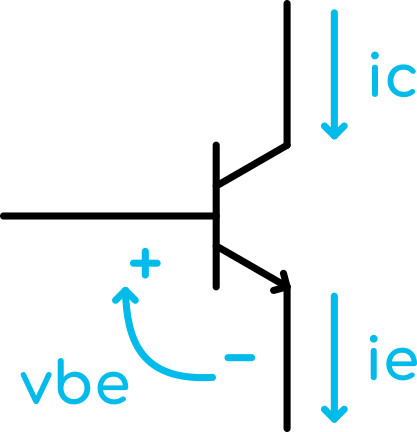
\includegraphics{circuits/single_transistor_circuit.png}
    \caption{BJT}
    \label{bjt}
\end{figure}

dove $V_T$ (o potenziale termico) e $I_s$ (o corrente di saturazione) sono variabili in
funzione della temperatura, anche se nella nostra analisi $V_T$ verrà considerato di
valore costante pari a $26\ mV$.

Per rimuovere dall'equazione $I_s$, che invece risulta molto più problematico, si collega
una coppia di transistor (idealmente nello stesso chip, in modo che siano il più possibile
simili tra loro e termicamente accoppiati) in configurazione differenziale:

\begin{figure}[H]
    \centering
    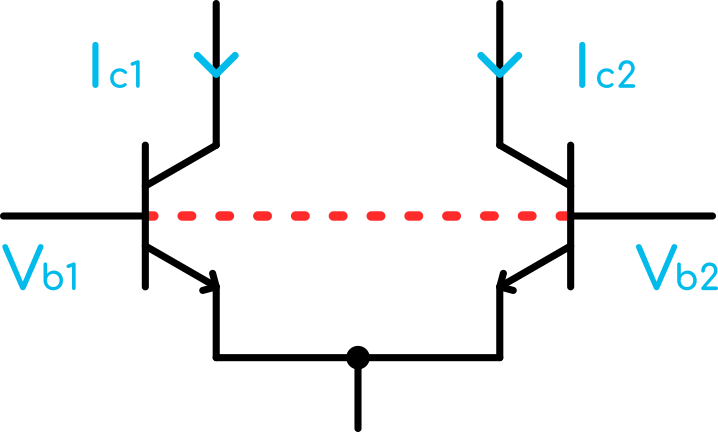
\includegraphics{circuits/differential_pair_circuit.png}
    \caption{Coppia differenziale a BJT}
    \label{differential_pair_circuit}
\end{figure}

per la quale possiamo scrivere la seguente relazione:

\begin{displaymath}
    \frac{I_{c2}}{I_{c1}}=\frac{I_s e^{\left(\frac{V_{be2}}{V_T}\right)}}{I_s e^{\left(\frac{V_{be1}}{V_T}\right)}}
    \qquad
    \rightarrow
    \qquad
    I_{c2}=I_{c1}e^{\left(\frac{V_{be2}-V_{be1}}{V_T}\right)}=I_{c1}e^{\left(\frac{V_{b2}-V_{b1}}{V_T}\right)}\ [A]
\end{displaymath}

in cui risulta evidente che la dipendenza da $I_s$ viene completamente rimossa.

A questo punto, rinominiamo le grandezze come segue:

\begin{displaymath}
    I_{freq}=I_{ref}e^{\left(-\frac{V_{b1}}{V_T}\right)}\ [A]
\end{displaymath}

e aggiungiamo al circuito

\begin{itemize}
    \item un amplificatore per portare $V_{in}$ in un range appropriato alla base di $Q_1$
          (operazionale di sinistra, figura \ref{exponential_converter_circuit})
          \begin{displaymath}
              V_{b1}=-V_{in}\cdot s=
              -V_{in}\cdot\frac{R_f}{R_{in}}\cdot\frac{\%R_{pot}+R}{R_{pot}+R}\ [V]
          \end{displaymath}
    \item un anello di controllo per mantenere la corrente di riferimento $I_{ref}$ costante
          (operazionale centrale, figura \ref{exponential_converter_circuit})
          \begin{displaymath}
              I_{ref}=\frac{V_{HR}-V_{LR}}{R_{ref}}\ [A]
          \end{displaymath}
    \item un convertitore corrente-tensione al collettore di $Q_2$ (operazionale di destra,
          figura \ref{exponential_converter_circuit})
          \begin{displaymath}
              V_{exp}=-I_{freq}\cdot R_{conv}\ [V]
          \end{displaymath}
\end{itemize}

ottenendo quindi il seguente circuito con la relativa relazione ingresso/uscita:

\begin{figure}[H]
    \centering
    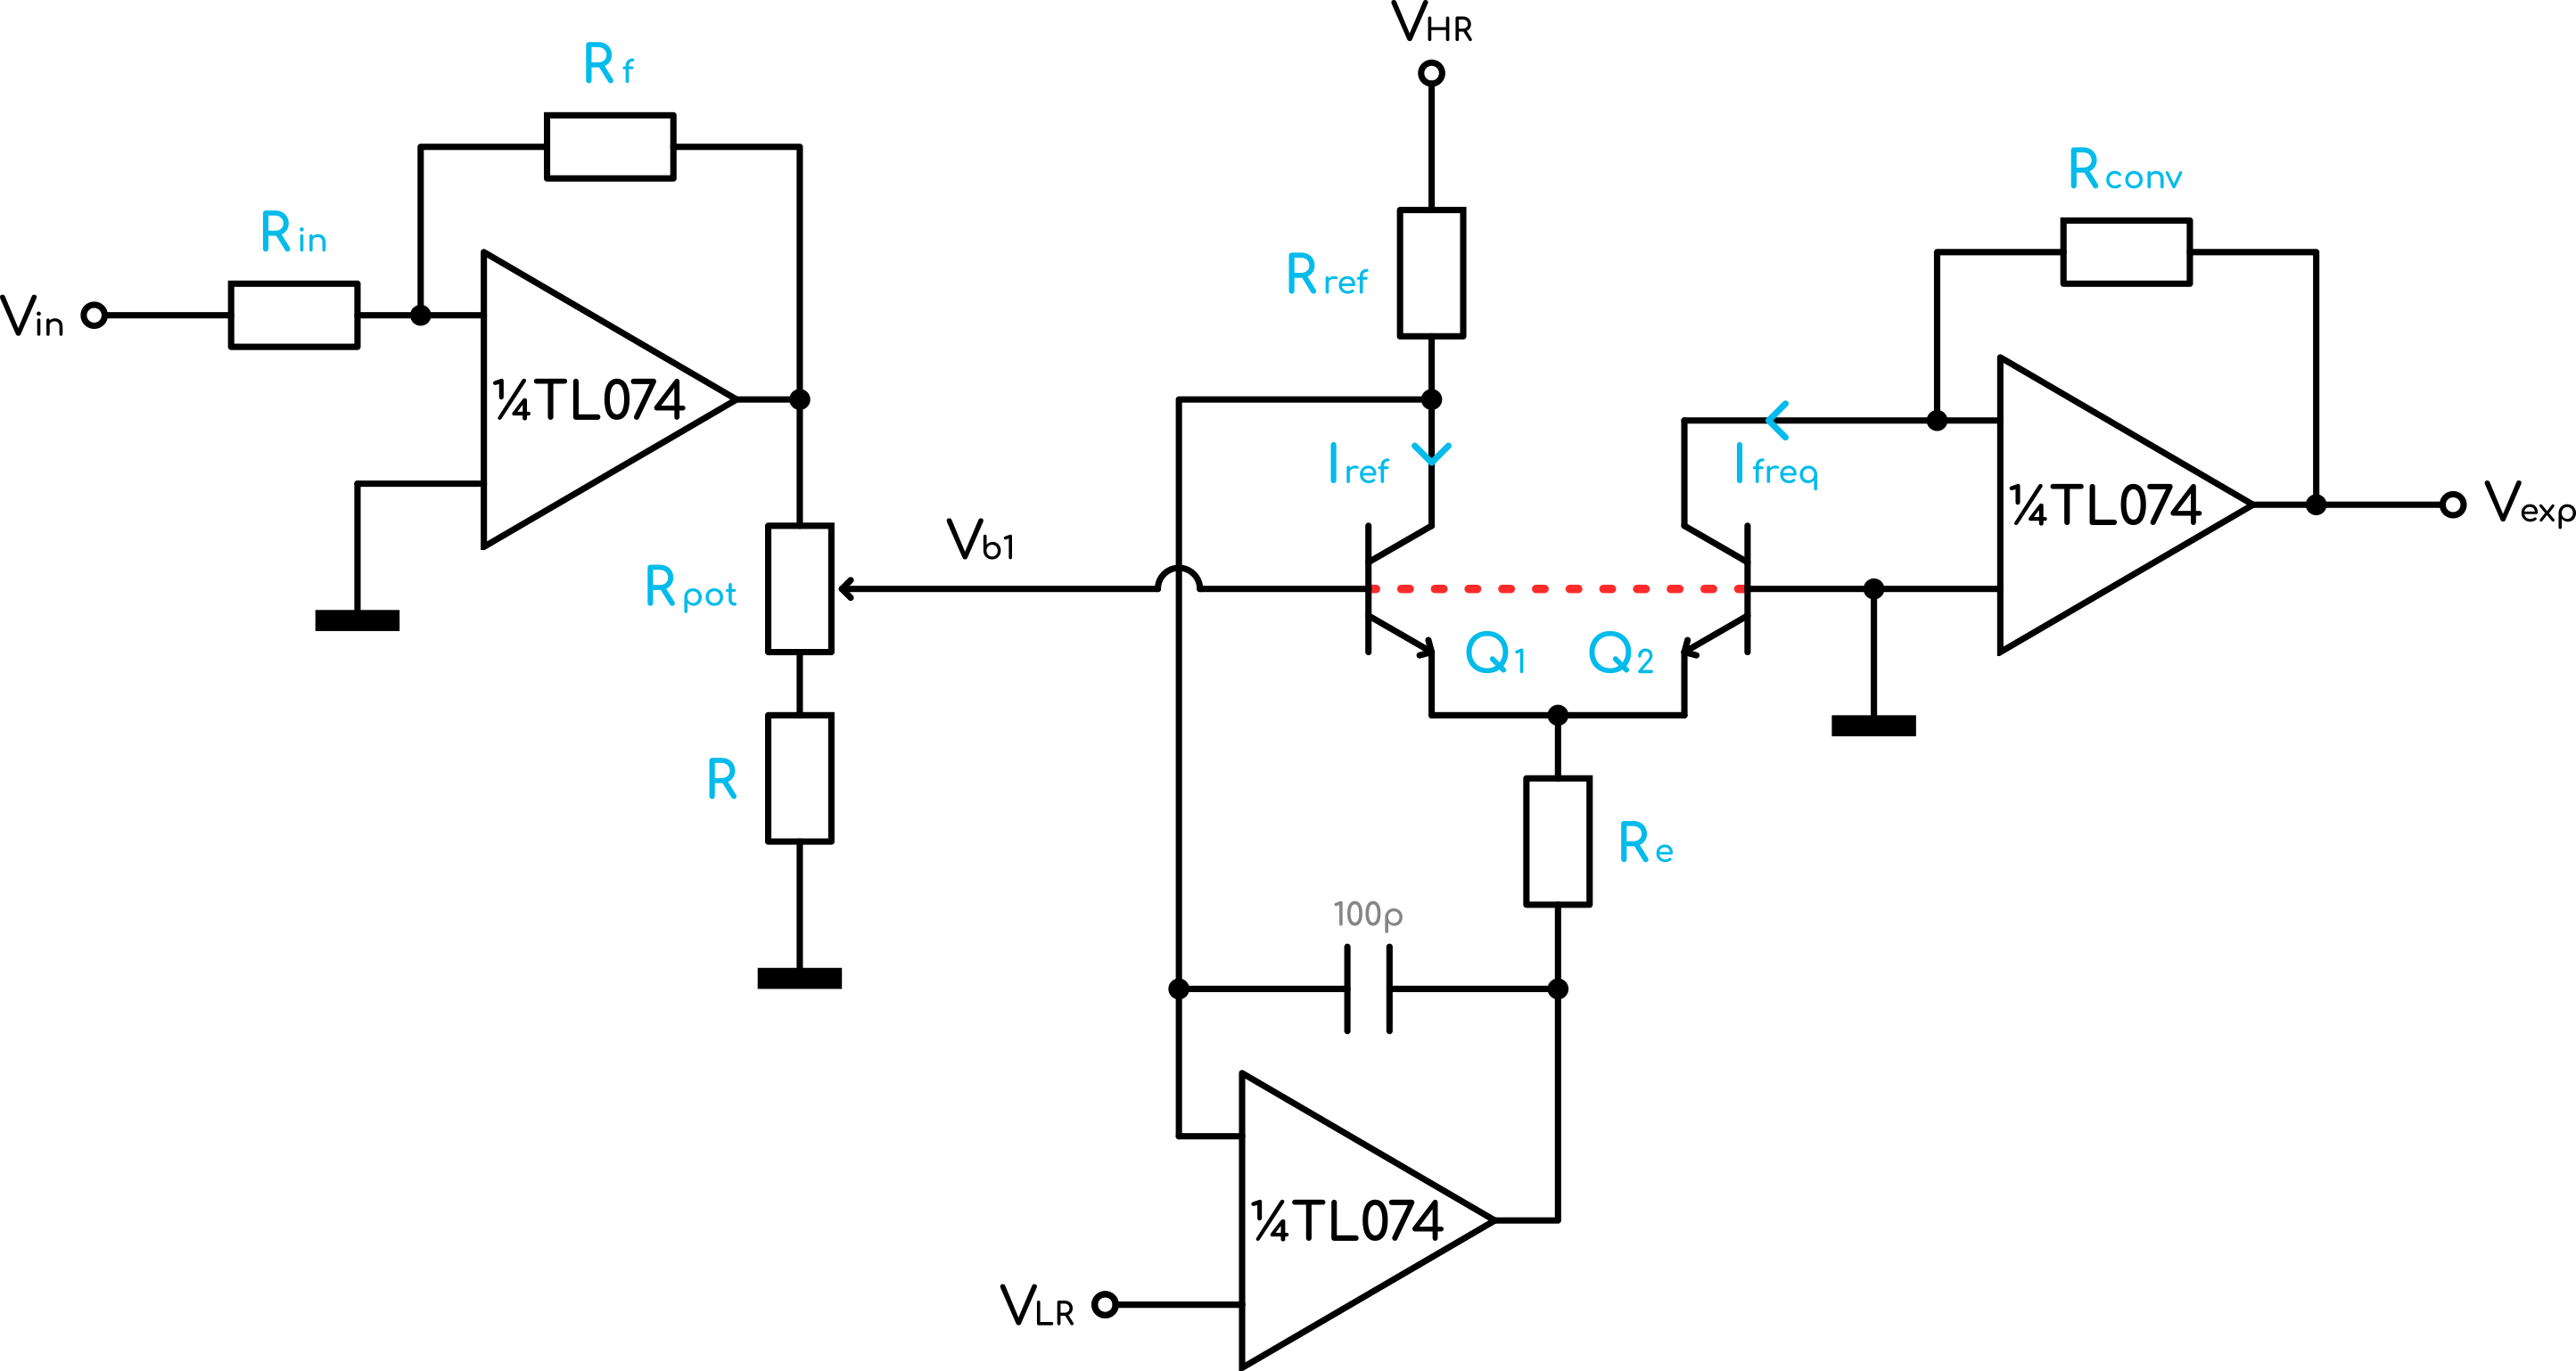
\includegraphics{circuits/exponential_converter_circuit.png}
    \caption{Schema elettrico del convertitore tensione lineare-esponenziale}
    \label{exponential_converter_circuit}
\end{figure}

\begin{displaymath}
    V_{exp}=R_f\cdot \frac{V_{HR}-V_{LR}}{R_{ref}}e^{\left(\frac{s\cdot V_{in}}{V_T}\right)}
\end{displaymath}

%--------------------------------------------------------------------------------------------

\subsection*{Dimensionamento e Scelta dei Componenti}

%--------------------------------------------------------------------------------------------

Passiamo quindi al dimensionamento dei componenti, in modo da imporre al circuito il
comportamento voluto.

Come prima cosa calcoliamo il valore del guadagno $s$ dell'amplificatore invertente.
Si vuole:

\begin{displaymath}
    I_{freq}=I_{ref}e^{\left(\frac{s\cdot V_{in}}{V_T}\right)}
    \qquad
    \rightarrow
    \qquad
    2I_{freq}=I_{ref}e^{\left(\frac{s\cdot(V_{in}+\Delta V_{in})}{V_T}\right)}
\end{displaymath}

qundi un raddoppio della corrente $I_{freq}$ per ogni variazione $\Delta V_{in}=1\ V$.
Allora possiamo riscrivere le due relazioni nel seguente modo:

\begin{displaymath}
    2=e^{\left(\frac{s\cdot\Delta V_{in}}{V_T}\right)}
    \qquad
    \rightarrow
    \qquad
    ln(2)=\frac{s\cdot\Delta V_{in}}{V_T}
    \qquad
    \rightarrow
    \qquad
    s=\frac{V_T\cdot ln(2)}{\Delta V_{in}}
\end{displaymath}

\begin{displaymath}
    s=\frac{26\ mV\cdot 0.6931}{1\ V}\approx0.018\approx\frac{1}{55.5}
\end{displaymath}

\begin{displaymath}
    s=\frac{R_f}{R_{in}}\cdot\frac{\%R_{pot}+R}{R_{pot}+R}
    =\frac{2\ k\Omega}{100\ k\Omega}\cdot\frac{440\ \Omega}{490\ \Omega}
    \approx 0.018
\end{displaymath}

quindi:

\begin{itemize}
    \item $R_f = 2\ k\Omega$;
    \item $R_{in} = 100\ k\Omega$;
    \item $R_{pot} = 100\ \Omega$;
    \item $R = 390\ \Omega$;
\end{itemize}

Scegliamo anche $R_{conv}=3.3\ k\Omega$, per avere come massimo valore di corrente
$I_{freq} = 3\ mA$ ($\approx+10\ V$ in uscita dal convertitore corrente-tensione),
in corrispondenza di una tensione di ingresso di $+8\ V$. Da qui possiamo quindi calcolare
il valore di $I_{ref}$:

\begin{displaymath}
    I_{ref}=I_{freq}e^{\left(-\frac{s\cdot V_{in}}{V_T}\right)}
    =0.003e^{\left(-\frac{0.018\cdot8}{0.026}\right)}
    \approx11.8\ \mu A
\end{displaymath}

Impostando quindi $V_{HR}=+12\ V$ e $V_{LR}=0\ V$ calcoliamo $R_{ref}$:

\begin{displaymath}
    R_{ref}=\frac{V_{HR}}{I_{ref}}=\frac{12}{11.8\cdot10^{-6}}\approx 1\ M\Omega
\end{displaymath}

Ora, poichè la corrente massima a scorrere in $R_e$ è la somma di $I_{ref}$ e $I_{freq}$
e quindi $\approx3\ \mu A$ possiamo scegliere anche $R_e=R_{conv}=3.3\ k\Omega$. In questo
modo sommando le cadute di potenziale $V_{R_{ref}}$, $V_{ce\_sat\_1}$ e $V_{R_e}$, siamo
dentro il limite dei valori di alimentazione, ottenendo $\approx 22.2\ V\ < 24\ V= 2V_{cc}$.

Tuttavia, qualora dovessero presentarsi problemi di saturazione prematura, è possibile
collegare un altro transistor in configurazione a diodo (o più semplicemente un diodo), per
ridurre la corrente che scorre nel ramo di $R_e$ e quindi la tensione ai suoi capi (in modo
non lineare). Il diodo infatti, non appena sufficientemente polarizzato, diventerebbe una
resistenza quasi nulla in parallelo ad una resistenza invece molto maggiore, questo accade
appena $V_{ce2}$ diventa maggiore di $\approx0.7\ V$.

\begin{figure}[H]
    \centering

    \begin{subfigure}{.5\textwidth}
        \centering
        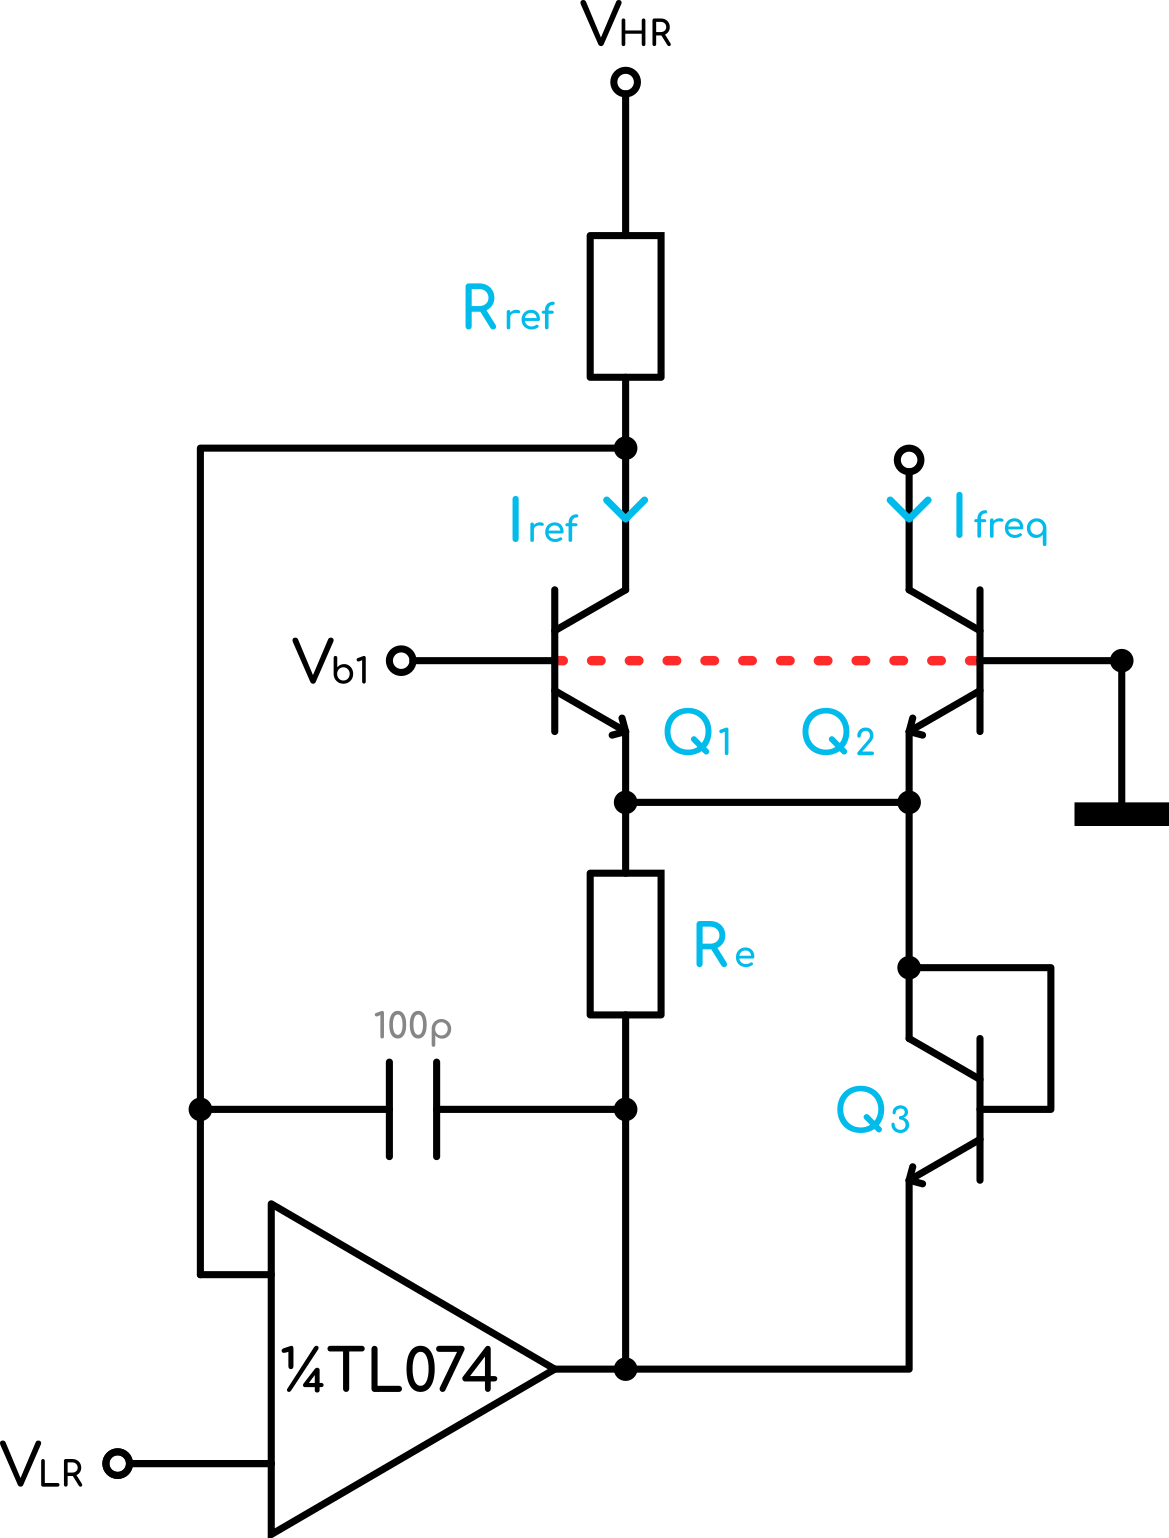
\includegraphics{circuits/expo_converter_transistor_circuit.png}
        \caption{Transistor in configurazione a diodo}
        \label{expo_converter_transistor_circuit}
    \end{subfigure}%
    \begin{subfigure}{.5\textwidth}
        \centering
        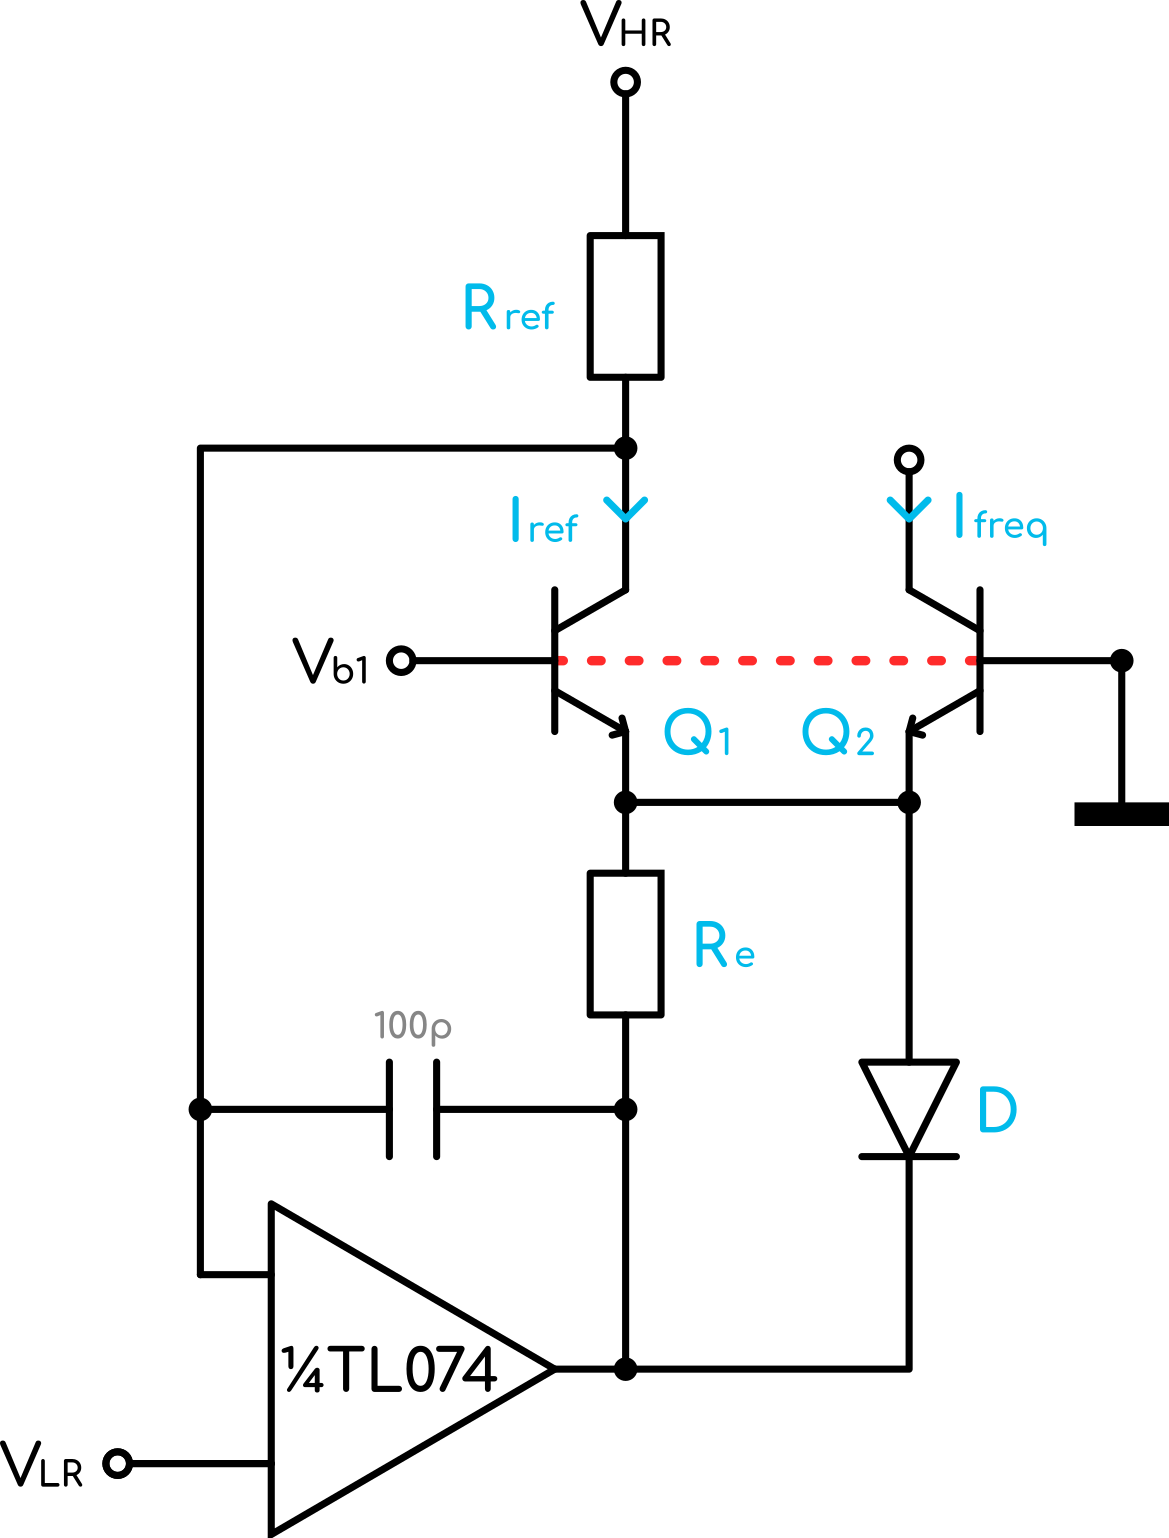
\includegraphics{circuits/expo_converter_diode_circuit.png}
        \caption{Diodo}
        \label{expo_converter_diode_circuit}
    \end{subfigure}

    \caption{Convertitori esponenziali con carico non-lineare}
    \label{non_linear_load_expo}
\end{figure}

Ancora una volta gli amplificatori operazionali utilizzati sono dei TL074, mentre si sceglie
un MPQ3904 \cite{mpq3904} per i transistor, chip che ospita 4 unità al proprio interno.

%--------------------------------------------------------------------------------------------

\subsection*{Risultati Pratici e Misure}

%--------------------------------------------------------------------------------------------

TODO misure e acquisizioni del convertitore lineare-esponenziale

%--------------------------------------------------------------------------------------------

\section{Somma di più Ingressi}

%--------------------------------------------------------------------------------------------

TODO descrizione sommatore

%--------------------------------------------------------------------------------------------

\section{Clipper}

%--------------------------------------------------------------------------------------------

TODO descrizione clipper

%--------------------------------------------------------------------------------------------

\subsection*{Risultati Pratici e Misure}

%--------------------------------------------------------------------------------------------

TODO misure e acquisizioni clipper

%--------------------------------------------------------------------------------------------
